\documentclass[UTF8]{ctexart}
%%%%%%%%%%%%%%%%%%%%%%%%%%%== 引入宏 ==%%%%%%%%%%%%%%%%%%%%%%%%%%%%%
\usepackage{cite}
\usepackage{amsmath}	% 使用数学公式
\usepackage{graphicx}	% 插入图片/PDF/EPS 等图像
\usepackage{subfigure}	% 使用子图像或者子表格
\usepackage{geometry}	% 设置页边距
\usepackage{fancyhdr}	% 设置页眉页脚
\usepackage{setspace}	% 设置行间距
\usepackage{hyperref}	% 让生成的文章目录有链接,点击时会自动跳转到该章节
\usepackage{url}
\usepackage{caption2}
\usepackage{authblk}
\usepackage{amsmath}
\usepackage{bm}
\graphicspath{{Figures/}}
\usepackage{appendix} % 附录
\usepackage{listings}
\usepackage{ctex}
\usepackage{pythonhighlight}

% 用来设置附录中代码的样式

\lstset{
	basicstyle          =   \sffamily,          % 基本代码风格
	keywordstyle        =   \bfseries,          % 关键字风格
	commentstyle        =   \rmfamily\itshape,  % 注释的风格,斜体
	stringstyle         =   \ttfamily,  % 字符串风格
	flexiblecolumns,                % 别问为什么,加上这个
	numbers             =   left,   % 行号的位置在左边
	showspaces          =   false,  % 是否显示空格,显示了有点乱,所以不现实了
	numberstyle         =   \zihao{-5}\ttfamily,    % 行号的样式,小五号,tt等宽字体
	showstringspaces    =   false,
	captionpos          =   t,      % 这段代码的名字所呈现的位置,t指的是top上面
	frame               =   lrtb,   % 显示边框
}

\lstdefinestyle{Python}{
	language        =   Python, % 语言选Python
	basicstyle      =   \zihao{-5}\ttfamily,
	numberstyle     =   \zihao{-5}\ttfamily,
	keywordstyle    =   \color{blue},
	keywordstyle    =   [2] \color{teal},
	stringstyle     =   \color{magenta},
	commentstyle    =   \color{red}\ttfamily,
	breaklines      =   true,   % 自动换行,建议不要写太长的行
	columns         =   fixed,  % 如果不加这一句,字间距就不固定,很丑,必须加
	basewidth       =   0.5em,
}

%%%%%%%%%%%%%%%%%%%%%%%%%%== 设置全局环境 ==%%%%%%%%%%%%%%%%%%%%%%%%%%%%
% [geometry] 设置页边距
\geometry{top=2.6cm, bottom=2.6cm, left=2.45cm, right=2.45cm, headsep=0.4cm, foot=1.12cm}
% 设置行间距为 1.5 倍行距
\onehalfspacing
% 设置页眉页脚
\pagestyle{fancy}
%\lhead{左头标}
%\chead{\today}
%\rhead{152xxxxxxxx}
\lfoot{}
\cfoot{\thepage}
\rfoot{}
%\renewcommand{\headrulewidth}{0.4pt}
%\renewcommand{\headwidth}{\textwidth}
%\renewcommand{\footrulewidth}{0pt}

%%%%%%%%%%%%%%%%%%%%%%%%%%== 自定义命令  ==%%%%%%%%%%%%%%%%%%%%%%%%%%%%%%
% 此行使文献引用以上标形式显示
\newcommand{\supercite}[1]{\textsuperscript{\cite{#1}}}
% 此行使section中的图、表、公式编号以A-B的形式显示
\renewcommand{\thetable}{\arabic{section}-\arabic{table}}
\renewcommand{\thefigure}{\arabic{section}-\arabic{figure}}
\renewcommand{\theequation}{\arabic{section}-\arabic{equation}}
% 此行使图注、表注与编号之间的分隔符缺省,默认是冒号:
\renewcommand{\captionlabeldelim}{~}

%===================================== 标题设置  ==========================================
% \heiti \kaishu 为字体设置,ctex 会自动根据操作系统加载字体
\title{\huge \CJKfamily{zhhei}基于慕测数据分析学生编程能力}	
\author{侯锐\textsuperscript{1} \quad 吴耀恩\textsuperscript{2} \quad 徐宇轩\textsuperscript{3}}
\affil{\small (\textsuperscript{1}{南京大学软件学院~软件工程~181250xxx}) \\ (\textsuperscript{2}{南京大学软件学院~软件工程~181250xxx}) \\ (\textsuperscript{2}{南京大学软件学院~软件工程~181250xxx})  }	
\date{} % 去除默认日期
%\date{\today}

%===================================== 正文区域  ==========================================
\begin{document}
	\maketitle
	
	\begin{flushleft}
		\textbf{摘要}:利用慕测平台一次编程作业的数据,运用一些数据处理方法,实现对于学生编程能力的评价\\[8pt]
		\textbf{关键词}:PCA,TOPSIS,题目难度,编程能力
	\end{flushleft}
	\section{研究问题}\label{sec1}
	
	\subsection{背景}
	随着人类社会技术的进步,编程逐渐成为信息科学一个基本知识和技能,成为一个跨专业、学科所必备的一个基本素养。很多高校现在更是把编程能力的培养作为理工科学生的必修课,随之流行起来的便是在线测评系统(OJ)。在线测评系统可以保存大量的测评数据,从中我们分析学习者的学习行为。本次研究就是基于慕测平台一次在线作业的数据,对参-+与该次作业的学生的编程能力做一次评价。
	
	\subsection{详细介绍}
	在本次研究中,一方面,我们通过主成分分析法(PCA)对数据中的题目做了分析,得到每个题目的难度系数,将难度系数与参与者对该题目的最终得分相结合,得到学生得分情况的测评;另一方面,我们通过xxxx(侯锐补充)的方法,对参与者提交的代码内容进行分析,得到学生代码书写情况的测评。考虑到不同的学生可能有不同的长处和喜好,分门别类的去评价一个学生的编程能力更加客观,我们针对每个学生,从字符串、树、图、排序等八个角度搜集学生的得分情况和代码情况,通过优劣解距离法(TOPSIS)实现对学生最终编程能力的打分。
	\subsection{应用场景}
	\label{sec1:subsec3}
	通过一次线上作业,老师对每类题型学生的掌握情况做一个大致的了解,方便改进和完善教学方法和促进与学生的沟通。作为学生,在完成一次作业后可以了解到自己与同期学生的差距在哪里,知道自己的优势和短处,有利于后期的学习和提高。
	
	
	\section{研究方法}\label{sec2}
	\subsection{数据集}
	基于慕测平台的提交记录数据,格式是json文件,内容包括每个参与者对每道题目的提交代码、最终得分、每次提交时间、每次提交得分等多个维度数据。通过学生id检索到具体学生,使用pythn提取数据,使用numpy,pandas,sklearn等工具分析。	
	
	\subsection{数据分析方法}
	
	\subsubsection{主成分分析法分析题目难度}
	\par (1)主成分分析法
	\par 主成分分析法也称主分量分析,是把多指标转化为少数几个综合指标,其中每个主成分都能够反映原始变量的大部分信息,主要用于数据降维。其步骤大致分为以下几步:
	\begin{itemize}
		\item 整理原始矩阵$X_{m \times n}$
		\item 求原始矩阵$X_{m \times n}$的协方差矩阵$S_{m \times n}$
		\item 求解协方差阵的特征值和特征向量
		\item 选取最大的$K$(人为给定)个特征值所对应的特征向量组成构成矩阵$W_{n \times k}$
		\item 最后计算$Z_{m \times k}=X_{m \times n}W_{n \times k}$
	\end{itemize}
	\par (2)维度的选取
	\par 根据已有的数据集,先要提取特征集。在提取特征之前,我们首先对数据集中的各个特征之间的关系进行了分析,选择出六个对编程题目难度研究最为有效的特征($X$)。
	\par
	\begin{enumerate}
		\item $X_1$:1A率
		\par 在寻找合适维度的过程中,我们首先考虑到的就是题目的AC数量。我们随机抽取了几道题目,发现不同的题目的AC数量有着较为明显的差异(见图x)。但是我们随即结合自身考虑到这样一种情况,:当一个同学在做练习时,最终运行出正确结果,但他对自己的解法并不满意,即通过了该题但是为了优化解题过程而去多次修改代码并提交通过,这样就提高了AC 量,使得这个特征不能那么客观地反映题目的难度类型。考虑到这个问题,我们最终选取1A率作为第一个维度,即一次通过的比率,用首次提交就通过的人数比总人数。
		\item $X_2$:AC率
		\par 用一道题目的通过人数比上总答题人数
		\item $X_3$:提交次数
		\par 一道题目的答题次数能反映这道题的难度
		\item $X_4$:最终平均分
		\par 每个同学提交成绩的最高分是这个题目的最终分,那么一道题目的最终分数的平均值可以反映这道题目在学生中的大体情况
		\item $X_5$:提交平均分
		\par 同学的每次提交都会得到一个及时反馈,将所有提交分数的均值作为另一个维度能一定程度上反映题目的难度
		\item $X_6$:Debug成效
		\par 部分同学最后一次提交突然变为0然后放弃debug,所以取最终得分而不是最后一次得分,另外也要假定同学做一道题途中不因该题过难而跳过去做另一道题然后过很久再倒回来的情况相对少见,而因题目过难而先跳过去的情况下时间会很长,因而也能反映题目难度。记一位同学最终得分$Score_{final}$,初次提交得分$Score_{first}$,最终提交时间$Time_{final}$,初次提交时间$Time_{first}$,那么
		$$X_6=\frac{Score_{final}-Score_{first}}{Time_{final}-Time_{first}}$$
	\end{enumerate}
	\par (3)数据处理与可视化
	\par 在决定最后保留几个维度的时候,我们首先通过不对n\_components赋值,此时默认返回min(X.shape)个特征,这样虽然没有减少特征个数,但是可以画出累计可解释方差贡献率曲线,以此选择最好的n\_components。累积可解释方差贡献率曲线是一条以降维后保留的特征个数为横坐标,降维后新特征矩阵捕捉到的可解释方差贡献率为纵坐标的曲线,能够帮助我们选择合适的维度。从图2-1可以看出来,选取二维或者三维的变化是不显著的。
	\begin{figure}[!htbp]
		\centering
		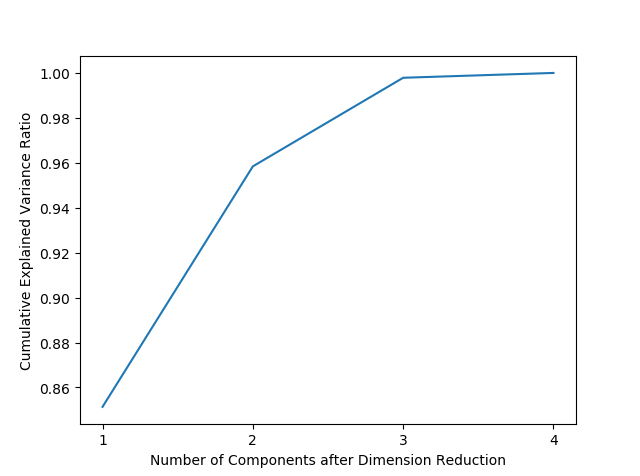
\includegraphics[width=0.35\textwidth]{Figure_2.png}\\
		\caption{累积可解释方差贡献率曲线}
	\end{figure}
	\par 最终PCA降维的结果如图2-2所示。
	\begin{figure}[!htbp]
		\centering
		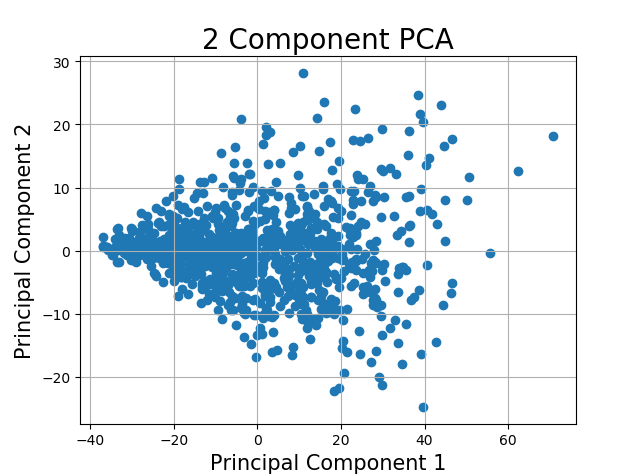
\includegraphics[width=0.35\textwidth]{Figure_1.png}\\
		\caption{降维后}
	\end{figure}
	\par 最后我们将两个维度加权求和,再将其指标正向化,并做标准化处理,得到一个(0,1)区间的系数,我们称为难度系数。我们随机抽取几道题目,如图所示,可见其难度系数是有显著差异的。
	\subsubsection{代码内容分析}
	\par (1)维度的选取
	\par 根据我们当初写python题的经验提取了3个能在一定程度上反映出代码水平的特征($X$):
	\par
	\begin{enumerate}
		\item $X_1$:代码规范性
		\par 代码的规范性能从一定程度上反映出一个人的代码的水平,渣的代码各有各的渣法,优雅的代码通常有共通之处。毕竟各路大神都比较强调这个。
		\par 具体做法:借助pylint库来检测每个同学每道题的代码并得到一个得分作为该道题代码规范性的分数,最终取平均值作为该同学的平均代码规范得分。
		\item $X_2$:if-elif-else与字面常量出现的次数
		\par 根据我们之前做这些练习题的经验,面向用例编程大概有两种不同的方向。简单点的是直接if-elif-else(这样if-elif-else出现的次数会比较多),复杂一点的就是把所有结果都放在列表里遍历列表然后用一个if-else即可判断出结果(这样if-else出现的次数少了但字面常量出现的次数会急剧上升),另一方面练习题并不是单靠简单的if-else的判断的堆积就能解出来的,字面常量的过多使用本身也不符合代码的编写规范,因此我们把这些的出现次数作为一个维度来评判代码的水平
		\par 具体做法:将一个学生做的所有题的代码都计算出次数并最终取平均作为该学生的最终次数
		\item $X_3$:非python代码的出现次数
		\par 由于我们是python练习题测试,那些直接复制粘贴网上的C++,Java代码(而不是弄懂代码逻辑后自己用python写一遍)且频率较高的学生的代码水平极大概率比较低,所以我们统计提交的非python代码的出现次数并将之作为一个维度
		\par 具体做法:$X_1$中当pylint库检测的代码非python代码时检测结果会报错,通过检索这种错误就能得知该代码是不是python代码。(我们发现properties文件记录的代码类型有少部分是错误的,所以没有直接用那个数据来统计)
	\end{enumerate}
	\par (2)数据的处理
	\par 由于选取的维度并不是直接从代码的算法上分析其水平而是从一些侧重点来反映代码水平,因此直接保留数据的绝大部分信息,降维表示代码的水平可能有失偏颇,误差较大。于是我们选取了损失信息来提高准确度的方式。仅根据这3个维度来将代码水平分成3类以期望获得较准确的结果。另一方面,物以类聚。相同代码水平的学生这些维度上表现相近的可能也较大。在分类的时候,我们最初的想法是直接分成高中低3类。但这样的话就要先选取部分学生的代码人工判定它是高水平还是低水平,然后再将剩余学生的代码的数据分析后往类里面塞。考虑到我们自己先来判定代码好坏的话主观因素过大,我们最终采取了另一种方式。利用数据间本身的相似特性来聚类,具有相似特征的数据如果能被聚成一类,然后我们再看这些类里的学生的代码普遍是高水平还是低水平,客观性就强多了。
	\par 最终我们使用KMeans算法来进行聚类分析,利用了sklearn里面的KMeans实现,将学生的代码水平分成高低3个档次,得到了一个学生id和其代码水平的字典。
	
	\subsubsection{优劣解距离法分析编程能力}
	\par(1)优劣解距离法
	\par C.L.Hwang 和 K.Yoon 于1981年首次提出 TOPSIS (Technique for Order Preference by Similarity to an Ideal Solution)。TOPSIS 法是一种常用的组内综合评价方法,能充分利用原始数据的信息,其结果能精确地反映各评价方案之间的差距。基本过程为基于归一化后的原始数据矩阵,采用余弦法找出有限方案中的最优方案和最劣方案,然后分别计算各评价对象与最优方案和最劣方案间的距离,获得各评价对象与最优方案的相对接近程度,以此作为评价优劣的依据。该方法对数据分布及样本含量没有严格限制,数据计算简单易行。其步骤大致分为以下几步:
	\begin{enumerate}
		\item 指标属性同向化
		\par TOPSIS 法使用距离尺度来度量样本差距,使用距离尺度就需要对指标属性进行同向化处理(若一个维度的数据越大越好,另一个维度的数据越小越好,会造成尺度混乱)。一般情况下会选择将极小型指标、中间型指标、区间型指标转化为极大型指标(数值越大评价越好),在本次研究中,数值均为该种情况,无需转化。
		\item 构造归一化矩阵
		\par 假设有n个评价对象,每个对象都有m个指标,则原始数据矩阵构造为:
		\begin{equation}
		\bm{X} =
		\begin{bmatrix}
		\bm{x_{11}} & \bm{x_{12}} & \cdots & \bm{x_{1m}} \\
		\bm{x_{21}} & \bm{x_{x_{22}}} & \cdots & \bm{x_{2m}} \\
		\vdots & \vdots &  \ddots & \vdots \\
		\bm{x_{n1}} & \bm{x_{n2}} & \cdots & \bm{x_{nm}}
		\end{bmatrix},
		\end{equation}
		构造加权规范矩阵,属性进行向量规范化,即每一列都除以当前列向量的范数:
		\begin{equation}
		Z_{ij}=\frac{x_{ij}}{\sqrt{\sum_{i=1}^n x_{ij}^2}}
		\end{equation}	
		由此得到归一化后的标准矩阵Z:
		\begin{equation}
		\bm{Z} =
		\begin{bmatrix}
		\bm{z_{11}} & \bm{z_{12}} & \cdots & \bm{z_{1m}} \\
		\bm{z_{21}} & \bm{x_{z_{22}}} & \cdots & \bm{z_{2m}} \\
		\vdots & \vdots &  \ddots & \vdots \\
		\bm{z_{n1}} & \bm{z_{n2}} & \cdots & \bm{z_{nm}}
		\end{bmatrix},
		\end{equation}
		\item 确定最优方案和最劣方案 \\
		最优方案 $\bm{Z^{+}}$由$\bm{Z}$中每列的最大值组成:
		\begin{equation}
		\bm{Z^{+}}=(\bm{max}\{z_{11},z_{21},\cdots,z_{n1}\},\bm{max}\{z_{12},z_{22},\cdots,z_{n2}\},\cdots,\bm{max}\{z_{1m},z_{2m},\cdots,z_{nm}\})
		=(Z_1^{+},Z_2^{+},\cdots,Z_m^{+})
		\end{equation}\\
		最劣方案 $\bm{Z^{-}}$由$\bm{Z}$中每列的最小值组成:
		\begin{equation}
		\bm{Z^{-}}=(\bm{min}\{z_{11},z_{21},\cdots,z_{n1}\},\bm{min}\{z_{12},z_{22},\cdots,z_{n2}\},\cdots,\bm{min}\{z_{1m},z_{2m},\cdots,z_{nm}\})=(Z_1^{-},Z_2^{-},\cdots,Z_m^{-})
		\end{equation}
		\item 计算各评价对象与最优方案和最劣方案的接近程度
		\begin{equation}
		\bm{D_i^{+}}=\sqrt{\sum_{j=1}^m {w_j(\bm{Z_j^{+}-z_{ij})^2}}}
		\end{equation}
		\begin{equation}
		\bm{D_i^{-}}=\sqrt{\sum_{j=1}^m {w_j(\bm{Z_j^{-}-z_{ij})^2}}}
		\end{equation}
		其中$w_j$是第$j$个属性的权重,本次研究采用人为确定的方法。
		\item 计算最终各个评价对象和最优方案的接近程度
		\begin{equation}
		\bm{C_i}=\frac{\bm{D_i^{-}}}{\bm{D_i^{-}}+\bm{D_i^{+}}}
		\end{equation}
		$0 \leq C_i \leq 1$,$C_i \rightarrow 1$ 表示评价对象越优秀
	\end{enumerate}
	\par (3)数据可视化
	\section{代码介绍}\label{sec3}
	\subsection{开源地址}
	\href{https://github.com/Coolingsky167/DataScienceHomework}{开源地址}
	\subsection{实现逻辑}
	
	
	
	\section{案例分析}\label{sec4}
	
	
	\section{意见和建议}\label{sec5}
	
	
	%===================================== 参考文献  ==========================================
	\section{参考文献}\label{sec:sec4}
	
	\begin{appendices} 
		\section{附录1} 
		\lstinputlisting[
		style       =   Python,
		caption     =   {\bf 主函数},
		label       =   {main.py}
		]{../../main.py}
		\section{附录2} 
		\lstinputlisting[
		style       =   Python,
		caption     =   {\bf TOPSIS},
		label       =   {TOPSIS.py}
		]{../../TOPSIS.py}
		\section{附录3} 
		\lstinputlisting[
		style       =   Python,
		caption     =   {\bf 获取数据},
		label       =   {.py}
		]{../../main.py}
	\end{appendices}
	
\end{document}